%%%%%%%%%%%%%%%%%%%%%%%%%%%%%%%%%%%%%%%%
% datoteka diploma-FRI-vzorec.tex
%
% vzorčna datoteka za pisanje diplomskega dela v formatu LaTeX
% na UL Fakulteti za računalništvo in informatiko
%
% na osnovi starejših verzij vkup spravil Franc Solina, maj 2021
% prvo verzijo je leta 2010 pripravil Gašper Fijavž
%
% za upravljanje z literaturo ta vezija uporablja BibLaTeX
%
% svetujemo uporabo Overleaf.com - na tej spletni implementaciji LaTeXa ta vzorec zagotovo pravilno deluje
%

\documentclass[a4paper,12pt,openright]{book}
%\documentclass[a4paper, 12pt, openright, draft]{book}  Nalogo preverite tudi z opcijo draft, ki pokaže, katere vrstice so predolge! Pozor, v draft opciji, se slike ne pokažejo!
 
\usepackage[utf8]{inputenc}   % omogoča uporabo slovenskih črk kodiranih v formatu UTF-8
\usepackage[slovene,english]{babel}    % naloži, med drugim, slovenske delilne vzorce
\usepackage[pdftex]{graphicx}  % omogoča vlaganje slik različnih formatov
\usepackage{fancyhdr}          % poskrbi, na primer, za glave strani
\usepackage{amssymb}           % dodatni matematični simboli
\usepackage{amsmath}           % eqref, npr.
\usepackage{hyperxmp}
\usepackage[hyphens]{url}
\usepackage{csquotes}
\usepackage{listings}
\renewcommand{\lstlistingname}{Izvorna koda}
\lstset{basicstyle=\footnotesize\ttfamily}

\usepackage[pdftex, colorlinks=true,
						citecolor=black, filecolor=black, 
						linkcolor=black, urlcolor=black,
						pdfproducer={LaTeX}, pdfcreator={LaTeX}]{hyperref}

\usepackage{color}
\usepackage{soul}

\usepackage[
backend=biber,
style=numeric,
sorting=nty,
]{biblatex}


\addbibresource{literatura.bib} %Imports bibliography file


%%%%%%%%%%%%%%%%%%%%%%%%%%%%%%%%%%%%%%%%
%	DIPLOMA INFO
%%%%%%%%%%%%%%%%%%%%%%%%%%%%%%%%%%%%%%%%
\newcommand{\ttitle}{Spletna aplikacija za glasbene festivale}
\newcommand{\ttitleEn}{Web application for music festivals}
\newcommand{\tsubject}{\ttitle}
\newcommand{\tsubjectEn}{\ttitleEn}
\newcommand{\tauthor}{Vasja Škarabot}
\newcommand{\tkeywords}{glasba, festival, socialno omrežje, spletna aplikacija}
\newcommand{\tkeywordsEn}{music, festival, social network, web application}

%%%%%%%%%%%%%%%%%%%%%%%%%%%%%%%%%%%%%%%%
%	HYPERREF SETUP
%%%%%%%%%%%%%%%%%%%%%%%%%%%%%%%%%%%%%%%%
\hypersetup{pdftitle={\ttitle}}
\hypersetup{pdfsubject=\ttitleEn}
\hypersetup{pdfauthor={\tauthor}}
\hypersetup{pdfkeywords=\tkeywordsEn}

%%%%%%%%%%%%%%%%%%%%%%%%%%%%%%%%%%%%%%%%
% postavitev strani
%%%%%%%%%%%%%%%%%%%%%%%%%%%%%%%%%%%%%%%%  

\addtolength{\marginparwidth}{-20pt} % robovi za tisk
\addtolength{\oddsidemargin}{40pt}
\addtolength{\evensidemargin}{-40pt}

\renewcommand{\baselinestretch}{1.3} % ustrezen razmik med vrsticami
\setlength{\headheight}{15pt}        % potreben prostor na vrhu
\renewcommand{\chaptermark}[1]%
{\markboth{\MakeUppercase{\thechapter.\ #1}}{}} \renewcommand{\sectionmark}[1]%
{\markright{\MakeUppercase{\thesection.\ #1}}} \renewcommand{\headrulewidth}{0.5pt} \renewcommand{\footrulewidth}{0pt}
\fancyhf{}
\fancyhead[LE,RO]{\sl \thepage} 
%\fancyhead[LO]{\sl \rightmark} \fancyhead[RE]{\sl \leftmark}
\fancyhead[RE]{\sc \tauthor}              % dodal Solina
\fancyhead[LO]{\sc Diplomska naloga}     % dodal Solina


\newcommand{\BibLaTeX}{{\sc Bib}\LaTeX}
\newcommand{\BibTeX}{{\sc Bib}\TeX}

%%%%%%%%%%%%%%%%%%%%%%%%%%%%%%%%%%%%%%%%
% naslovi
%%%%%%%%%%%%%%%%%%%%%%%%%%%%%%%%%%%%%%%%  

\newcommand{\autfont}{\Large}
\newcommand{\titfont}{\LARGE\bf}
\newcommand{\clearemptydoublepage}{\newpage{\pagestyle{empty}\cleardoublepage}}
\setcounter{tocdepth}{1}	      % globina kazala

%%%%%%%%%%%%%%%%%%%%%%%%%%%%%%%%%%%%%%%%
% konstrukti
%%%%%%%%%%%%%%%%%%%%%%%%%%%%%%%%%%%%%%%%  
\newtheorem{izrek}{Izrek}[chapter]
\newtheorem{trditev}{Trditev}[izrek]
\newenvironment{dokaz}{\emph{Dokaz.}\ }{\hspace{\fill}{$\Box$}}


%%%%%%%%%%%%%%%%%%%%%%%%%%%%%%%%%%%%%%%%%%%%%%%%%%%%%%%%%%%%%%%%%%%%%%%%%%%%%%%
%% PDF-A
%%%%%%%%%%%%%%%%%%%%%%%%%%%%%%%%%%%%%%%%%%%%%%%%%%%%%%%%%%%%%%%%%%%%%%%%%%%%%%%

%%%%%%%%%%%%%%%%%%%%%%%%%%%%%%%%%%%%%%%% 
% define medatata
%%%%%%%%%%%%%%%%%%%%%%%%%%%%%%%%%%%%%%%% 
\def\Title{\ttitle}
\def\Author{\tauthor, vs7015@student.uni-lj.si}
\def\Subject{\ttitleEn}
\def\Keywords{\tkeywordsEn}

%%%%%%%%%%%%%%%%%%%%%%%%%%%%%%%%%%%%%%%% 
% \convertDate converts D:20080419103507+02'00' to 2008-04-19T10:35:07+02:00
%%%%%%%%%%%%%%%%%%%%%%%%%%%%%%%%%%%%%%%% 
\def\convertDate{%
    \getYear
}

{\catcode`\D=12
 \gdef\getYear D:#1#2#3#4{\edef\xYear{#1#2#3#4}\getMonth}
}
\def\getMonth#1#2{\edef\xMonth{#1#2}\getDay}
\def\getDay#1#2{\edef\xDay{#1#2}\getHour}
\def\getHour#1#2{\edef\xHour{#1#2}\getMin}
\def\getMin#1#2{\edef\xMin{#1#2}\getSec}
\def\getSec#1#2{\edef\xSec{#1#2}\getTZh}
\def\getTZh +#1#2{\edef\xTZh{#1#2}\getTZm}
\def\getTZm '#1#2'{%
    \edef\xTZm{#1#2}%
    \edef\convDate{\xYear-\xMonth-\xDay T\xHour:\xMin:\xSec+\xTZh:\xTZm}%
}

%\expandafter\convertDate\pdfcreationdate 

%%%%%%%%%%%%%%%%%%%%%%%%%%%%%%%%%%%%%%%%
% get pdftex version string
%%%%%%%%%%%%%%%%%%%%%%%%%%%%%%%%%%%%%%%% 
\newcount\countA
\countA=\pdftexversion
\advance \countA by -100
\def\pdftexVersionStr{pdfTeX-1.\the\countA.\pdftexrevision}


%%%%%%%%%%%%%%%%%%%%%%%%%%%%%%%%%%%%%%%%
% XMP data
%%%%%%%%%%%%%%%%%%%%%%%%%%%%%%%%%%%%%%%%  
\usepackage{xmpincl}
%\includexmp{pdfa-1b}

%%%%%%%%%%%%%%%%%%%%%%%%%%%%%%%%%%%%%%%%
% pdfInfo
%%%%%%%%%%%%%%%%%%%%%%%%%%%%%%%%%%%%%%%%  
\pdfinfo{%
    /Title    (\ttitle)
    /Author   (\tauthor, vs7015@student.uni-lj.si)
    /Subject  (\ttitleEn)
    /Keywords (\tkeywordsEn)
    /ModDate  (\pdfcreationdate)
    /Trapped  /False
}

%%%%%%%%%%%%%%%%%%%%%%%%%%%%%%%%%%%%%%%%
% znaki za copyright stran
%%%%%%%%%%%%%%%%%%%%%%%%%%%%%%%%%%%%%%%%  

\newcommand{\CcImageCc}[1]{%
	
\includegraphics[scale=#1]{cc_cc_30.pdf}%
}
\newcommand{\CcImageBy}[1]{%
	
\includegraphics[scale=#1]{cc_by_30.pdf}%
}
\newcommand{\CcImageSa}[1]{%
	
\includegraphics[scale=#1]{cc_sa_30.pdf}%
}

%%%%%%%%%%%%%%%%%%%%%%%%%%%%%%%%%%%%%%%%%%%%%%%%%%%%%%%%%%%%%%%%%%%%%%%%%%%%%%%
%%%%%%%%%%%%%%%%%%%%%%%%%%%%%%%%%%%%%%%%%%%%%%%%%%%%%%%%%%%%%%%%%%%%%%%%%%%%%%%

\begin{document}
\selectlanguage{slovene}
\frontmatter
\setcounter{page}{1} %
\renewcommand{\thepage}{}       % preprečimo težave s številkami strani v kazalu

%%%%%%%%%%%%%%%%%%%%%%%%%%%%%%%%%%%%%%%%
%naslovnica
 \thispagestyle{empty}%
   \begin{center}
    {\large\sc Univerza v Ljubljani\\%
%      Fakulteta za elektrotehniko\\% za študijski program Multimedija
%      Fakulteta za upravo\\% za študijski program Upravna informatika
      Fakulteta za računalništvo in informatiko\\%
%      Fakulteta za matematiko in fiziko\\% za študijski program Računalništvo in matematika
     }
    \vskip 10em%
    {\autfont \tauthor\par}%
    {\titfont \ttitle \par}%
    {\vskip 3em \textsc{DIPLOMSKO DELO\\[5mm]         % dodal Solina za ostale študijske programe
    VISOKOŠOLSKI STROKOVNI ŠTUDIJSKI PROGRAM\\ PRVE STOPNJE\\ RAČUNALNIŠTVO IN INFORMATIKA}\par}%
%     UNIVERZITETNI  ŠTUDIJSKI PROGRAM\\ PRVE STOPNJE\\ RAČUNALNIŠTVO IN INFORMATIKA}\par}%
%    INTERDISCIPLINARNI UNIVERZITETNI\\ ŠTUDIJSKI PROGRAM PRVE STOPNJE\\ MULTIMEDIJA}\par}%
%    INTERDISCIPLINARNI UNIVERZITETNI\\ ŠTUDIJSKI PROGRAM PRVE STOPNJE\\ UPRAVNA INFORMATIKA}\par}%
%    INTERDISCIPLINARNI UNIVERZITETNI\\ ŠTUDIJSKI PROGRAM PRVE STOPNJE\\ RAČUNALNIŠTVO IN MATEMATIKA}\par}%
    \vfill\null%
% izberite pravi habilitacijski naziv mentorja!
    {\large \textsc{Mentor}: viš. pred. dr. Aljaž Zrnec\par}%
    {\vskip 2em \large Ljubljana, \the\year \par}%
\end{center}
% prazna stran
%\clearemptydoublepage      
% izjava o licencah itd. se izpiše na hrbtni strani naslovnice

%%%%%%%%%%%%%%%%%%%%%%%%%%%%%%%%%%%%%%%%
%copyright stran
%%%%%%%%%%%%%%%%%%%%%%%%%%%%%%%%%%%%%%%%
\newpage
\thispagestyle{empty}

\vspace*{5cm}
{\small \noindent
To delo je ponujeno pod licenco \textit{Creative Commons Priznanje avtorstva-Deljenje pod enakimi pogoji 2.5 Slovenija} (ali novej\v so razli\v cico).
To pomeni, da se tako besedilo, slike, grafi in druge sestavine dela kot tudi rezultati diplomskega dela lahko prosto distribuirajo,
reproducirajo, uporabljajo, priobčujejo javnosti in predelujejo, pod pogojem, da se jasno in vidno navede avtorja in naslov tega
dela in da se v primeru spremembe, preoblikovanja ali uporabe tega dela v svojem delu, lahko distribuira predelava le pod
licenco, ki je enaka tej.
Podrobnosti licence so dostopne na spletni strani \href{http://creativecommons.si}{creativecommons.si} ali na Inštitutu za
intelektualno lastnino, Streliška 1, 1000 Ljubljana.

\vspace*{1cm}
\begin{center}% 0.66 / 0.89 = 0.741573033707865
\CcImageCc{0.741573033707865}\hspace*{1ex}\CcImageBy{1}\hspace*{1ex}\CcImageSa{1}%
\end{center}
}

\vspace*{1cm}
{\small \noindent
Izvorna koda diplomskega dela, njeni rezultati in v ta namen razvita programska oprema je ponujena pod licenco GNU General Public License,
različica 3 (ali novejša). To pomeni, da se lahko prosto distribuira in/ali predeluje pod njenimi pogoji.
Podrobnosti licence so dostopne na spletni strani \url{http://www.gnu.org/licenses/}.
}

\vfill
\begin{center} 
\ \\ \vfill
{\em
Besedilo je oblikovano z urejevalnikom besedil \LaTeX.}
\end{center}

% prazna stran
\clearemptydoublepage

%%%%%%%%%%%%%%%%%%%%%%%%%%%%%%%%%%%%%%%%
% stran 3 med uvodnimi listi
\thispagestyle{empty}
\
\vfill

\bigskip
\noindent\textbf{Kandidat:} Vasja Škarabot\\
\noindent\textbf{Naslov:} Spletna aplikacija za glasbene festivale\\
% vstavite ustrezen naziv študijskega programa!
\noindent\textbf{Vrsta naloge:} Diplomska naloga na visokošolskem programu prve stopnje Računalništvo in informatika \\
% izberite pravi habilitacijski naziv mentorja!
\noindent\textbf{Mentor:} viš. pred. dr. Aljaž Zrnec\\

\bigskip
\noindent\textbf{Opis:}\\
Besedilo teme diplomskega dela študent prepiše iz študijskega informacijskega sistema, kamor ga je vnesel mentor. 
V nekaj stavkih bo opisal, kaj pričakuje od kandidatovega diplomskega dela. 
Kaj so cilji, kakšne metode naj uporabi, morda bo zapisal tudi ključno literaturo.

\bigskip
\noindent\textbf{Title:} Web application for music festivals

\bigskip
\noindent\textbf{Description:}\\
opis diplome v angleščini

\vfill



\vspace{2cm}

% prazna stran
\clearemptydoublepage

% zahvala
\thispagestyle{empty}\mbox{}\vfill\null\it%
\noindent
Na tem mestu zapišite, komu se zahvaljujete za pomoč pri izdelavi diplomske naloge oziroma pri vašem študiju nasploh. Pazite, da ne boste koga pozabili. Utegnil vam bo zameriti. Temu se da izogniti tako, da celotno zahvalo izpustite.
\rm\normalfont

% prazna stran
\clearemptydoublepage


%%%%%%%%%%%%%%%%%%%%%%%%%%%%%%%%%%%%%%%%
% kazalo
\pagestyle{empty}
\def\thepage{}% preprečimo težave s številkami strani v kazalu
\tableofcontents{}


% prazna stran
\clearemptydoublepage

%%%%%%%%%%%%%%%%%%%%%%%%%%%%%%%%%%%%%%%%
% seznam kratic

\chapter*{Seznam uporabljenih kratic}

\noindent\begin{tabular}{p{0.11\textwidth}|p{.39\textwidth}|p{.39\textwidth}}    % po potrebi razširi prvo kolono tabele na račun drugih dveh!
  {\bf kratica} & {\bf angleško}                              & {\bf slovensko} \\ \hline
  {\bf API}      & Application Programming Interface               & Aplikacijski programski vmesnik \\
  {\bf DBMS} & database management system & sistem za upravljanje podatkovnih baz \\
  {\bf SVM}   & support vector machine              & metoda podpornih vektorjev \\
%  \dots & \dots & \dots \\
\end{tabular}


% prazna stran
\clearemptydoublepage

%%%%%%%%%%%%%%%%%%%%%%%%%%%%%%%%%%%%%%%%
% povzetek
\phantomsection
\addcontentsline{toc}{chapter}{Povzetek}
\chapter*{Povzetek}

\noindent\textbf{Naslov:} \ttitle
\bigskip

\noindent\textbf{Avtor:} \tauthor
\bigskip

%\noindent\textbf{Povzetek:} 
\noindent 
Diplomska naloga predstavlja razvoj in implementacijo spletne aplikacije za glasbene festivale. Glavni namen aplikacije je, uporabnikom olajšati
dostop do vseh pomembnih informacij, ter jim omogočiti medsebojno komunikacijo in preko le te graditi skupnosti s pomočjo forumov in klepetov. 

Spletna aplikacija uporabniku omogoča pregled nad festivali, vključno z iskanjem prenočišč v bližini ter navodili za pot do prizorišča, forum na katerem lahko uporabniki
objavljajo novice, delijo nasvete ter postavljajo morebitna vprašanja, ki se jim porajajo, ter klepeti, katere lahko uporabniki uporabijo z namenom razpravljanja in dogovarjanja za skupni obisk. 

Za implementacijo čelnega dela smo uporabili ogrodje Nuxt.js, za zaledni del pa Django z razširitvijo Rest Framework in podatkovno bazo PostgreSQL. Vse skupaj poganjamo v Dockerju.
Zemljevidi so implementirani s pomočjo platforme Mapbox, realnočasovno komunikacijo v klepetih omogoča Pusher, slike pa shranjujemo s pomočjo Firebase shrambe.

\bigskip

\noindent\textbf{Ključne besede:} \tkeywords.
% prazna stran
\clearemptydoublepage

%%%%%%%%%%%%%%%%%%%%%%%%%%%%%%%%%%%%%%%%
% abstract
\phantomsection
\selectlanguage{english}
\addcontentsline{toc}{chapter}{Abstract}
\chapter*{Abstract}

\noindent\textbf{Title:} \ttitleEn
\bigskip

\noindent\textbf{Author:} \tauthor
\bigskip

%\noindent\textbf{Abstract:} 
\noindent 
The thesis presents the development and implementation of a web application for music festivals. The main purpose of the application is to make it easier for users
access to all relevant information, and to allow users to communicate with each other and build communities through forums and chats. 

The web application provides the user with an overview of the festivals, including a search for nearby accommodation and directions to the venue, a forum where users can
post news, share tips and ask any questions they may have, and chat rooms which users can use to discuss and arrange to visit together. 

For the front-end implementation, we used the Nuxt.js framework, and for the back-end we used Django with the Rest Framework extension and the PostgreSQL database. 
We run everything inside Docker containers. Maps are implemented using the Mapbox platform, real-time communication in chats is enabled by Pusher, and images are stored using the Firebase Storage.

\bigskip

\noindent\textbf{Keywords:} \tkeywordsEn.
\selectlanguage{slovene}
% prazna stran
\clearemptydoublepage

%%%%%%%%%%%%%%%%%%%%%%%%%%%%%%%%%%%%%%%%
\mainmatter
\setcounter{page}{1}
\pagestyle{fancy}

\chapter{Uvod}
\section{Motivacija}
Vsako leto veliko ljudi obišče kakšen glasbeni festival. Pridobivanje informacij in samo načrtovanje obiska pa lahko kar hitro postane nadležno, 
in posledično lahko hitro pokvari uporabniško izkušnjo, že pred samim obiskom festivala.
Najprej se uporabnik odloči za enega izmed festivalov.
Ponavadi to stori na podlagi različnih dejavnikov, kot so cena, lokacija in datum poteka, veliko pa pomenijo tudi predhodne izkušnje ostalih.
Problem pa je, da je potrebno vse te informacije iskati po različnih spletnih straneh saj rešitve, s katero bi lahko pridobili vse informacije na enem mestu ni. 
Poleg tega bi bilo smiselno implementirati rešitev, kjer si lahko uporabniki medesebojno pomagajo, 
s tem da delijo predhodne izkušnje, novosti in mnenja v obliki foruma ali pa morda celo dobijo nove prijatelje, v živo razpravljajo in mogoče nekoč celo skupaj
obiščejo kakšen festival s pomočjo klepetov v živo. 

\section{Cilji}
Cilj diplomske naloge je torej razviti spletno aplikacijo, ki bo uporabnikom olajšala iskanje glasbenih festivalov in udeležbo na njih, 
ustvariti skupnost, v kateri lahko uporabniki izmenjujejo izkušnje, nasvete in novice,
ter vzpodbuditi interakcijo med obiskovalci festivala v živo, ter s tem izboljšati festivalsko izkušnjo.

\section{Struktura diplomske naloge}

% TODO poglej si kaj je ref{}


\chapter{Obstoječe rešitve}
V uporabi trenutno ni nobene podobne rešitve, zaradi česar se obiskovalci festivalov poslužujejo različnih aplikacij in spletnih strani. 
Za postavljanje vprašanj sta to običajno Reddit ali pa Tripadvisor. Ti rešitvi nista primarno namenjeni glasbenim festivalom, 
zato težko najdemo koristne podatke, saj vsebujeta le forume za večje festivale.
Poleg tega mora vsak uporabljati več aplikacij za različne namene in zato nimamo vsega na eni platformi. Uporabnik mora tako npr. za iskanje informacij o festivalu najprej na spletno stran festivala,
nato prebira različne forume (Reddit, Tripadvisor), zraven tega še išče prenočišča na Bookingu, potem pa se še na tretji platformi z ostalimi pogovarja/dogovarja (npr. Messenger).
V tem poglavju bodo opisane naštete alternative, njihove prednosti in slabosti.

\section{Tripadvisor}
Tripadvisor je spletna platforma za iskanje prenočišč \cite{tripadvisor}. Je ena večjih platform namenjenih planiranju potovanj, ki uporabnikom omogoča tudi podajanje kritik in ocen.

\begin{itemize}
    \item Prednosti:
        \begin{itemize}
            \item Velik nabor uporabnikov in posledično kritik in ocen za prenočišča in razne dogodke.
            \item Širok nabor funkcionalnosti. Poleg osnovnih funkcionalnosti še orodja za načrtovanje poti, vodniki in priporočila.
        \end{itemize}
    \item Slabosti:
        \begin{itemize}
            \item Vsebuje le najpopularnejše festivale.
            \item Ocene bolj osredotočene na nastanitve in potovanje kot na sam festival.
            \item Ne vsebuje nekaterih pomembnih informacij, kot so datumi, informacije o cenah in izvajalcih.
            \item Uporabnik lahko z ostalimi uporabniki komunicira le posredno preko foruma. Za neposredno komunikacijo se mora poslužiti drugih platform.
        \end{itemize}
\end{itemize}

\section{Reddit}
Reddit je forumsko socialno omrežje, kjer lahko uporabniki objavljajo, ostali pa nato te objave komentirajo in glasujejo \cite{reddit}. Objave so razvrščene v podstrani imenovane subredditi oz. skupnosti.
Na Redditu najdemo skupnosti za nekatere glasbene festivale, kjer se uporabniki obveščajo o novicah o festivalu in podajajo različna vprašanja. Je pa teh skupnosti precej malo, še tiste ki so, 
pa so po večini skupnosti največjih glasbenih festivalov na svetu (Coachella, Tomorrowland, UMF).

\begin{itemize}
    \item Prednosti:
        \begin{itemize}
            \item Pri večjih festivalih ogromen nabor vprašanj, razprav, nasvetov in novic.
            \item Možnost realno-časovne komunikacije z ostalimi.
        \end{itemize}
    \item Slabosti:
        \begin{itemize}
            \item Večino osnovnih informacij mora uporabnik pridobiti na ostalih straneh.
            \item Težko je najti skupnosti, ki niso namenjene le največjim festivalom.
            \item Čeprav lahko uporabniki komunicirajo v realnem času, lahko to počnejo le v privatnih skupinah, ki niso del subredditov.
        \end{itemize}
\end{itemize}

\section{Woov}
Woov je namenska aplikacija za obiskovalce glasbenih festivalov~\cite{woov}. Povezani so z več kot 1000 dogodki po 40 državah, uporabnikom pa omogočajo vpogled v časovnice, zemljevid prizorišč in komunikacijo z ostalimi uporabniki.
Namen aplikacije je pomagati obiskovalcem, ki so že na prizorišču.

\begin{itemize}
    \item Prednosti:
        \begin{itemize}
            \item Uporabniki lahko aplikacijo prenesejo na telefon.
            \item Pomembne informacije kot so datumi, prizorišče, nastopajoči izvajalci.
            \item Uporabniki si lahko pomagajo z zemljevidom, ki vključuje lokacije stojnic, wc-jev, odrov in polnilnih postaj.
            \item Realno-časovna komunikacija.
        \end{itemize}
    \item Slabosti:
        \begin{itemize}
            \item Dogodki so običajno dodani nekaj dni pred začetkom festivala. Posledično si uporabnik za planiranje ne more dosti pomagati.
            \item Aplikacija včasih deluje nelogična za nove uporabnike, saj so nekatere funkcionalnosti precej skrite.
            \item Uporabniki ne morejo podati svojih mnenj.
            \item Aplikaciji lahko prispevajo le partnerji. To ni nujno slabo, vendar omeji aplikacije le na določene festivale.
        \end{itemize}
\end{itemize}

% NOVO POGLAVJE
\chapter{Zajem zahtev}
Preden smo sploh začeli z načrtovanjem podatkovne baze in kodiranjem, je bilo potrebno definirati vse naloge, ki jih bo sistem opravljal.
S tem smo si zadali načrt in ogrodje, kateremu smo pri razvoju nato sledili.
Z dobro definicijo zahtev smo dosegli to, da smo zmanjšali verjetnost pomembnih sprememb med razvojem, s čimer smo prihranili čas in trud.

\section{Funkcionalnosti sistema}
Naša aplikacija mora uporabniku omogočiti:
\begin{itemize}
    \item Registracijo in prijavo.
    \item Pregled nad glasbenimi festivali z možnostjo iskanja in filtriranja.
    \item Dodajanje festivalov in dodelitev moderatorskih pravic.
    \item Izpis podrobnosti glasbenega festivala, vključno z datumi, žanri in povezavo do uradne spletne strani.
    \item Pogled na zemljevid z lokacijo glasbenega festivala, ki se lahko razširi v navodila za pot.
    \item Iskanje prenočišč v okolici glasbenega festivala glede na podane parametre.
    \item Branje objav z možnostjo filtriranja in iskanja na forumu za določen festival.
    \item Objavljanje na forumih.
    \item Všečkanje in komentiranje objav.
    \item Dodajanje javnih klepetov za festivale.
    \item Pošiljanje sporočil v klepetih.
    \item Naročanje na obvestila za klepete ob novih sporočilih.
\end{itemize}

Moderatorji pa lahko povrh vsega še:
\begin{itemize}
    \item Urejajo podatke za svoje festivale.
    \item Brišejo neprimerne objave.
    \item Brišejo neprimerne komentarje.
\end{itemize}

\section{Diagram primerov uporabe}
Na Sliki~\ref{usecase} je prikazan diagram primerov uporabe za našo aplikacijo. 
V diagramu nastopata 2 akterja in sicer Uporabnik in Moderator.
Iz diagrama je razvidno, kaj lahko oba tipa uporabnikov v aplikaciji počneta.
Podrobneje pa bomo delovanje aplikacije predstavili v poglavju~\ref{UI}.

\begin{figure}[p] % OPTIONS h-here, t-top, b-bottom, p-page
\begin{center}
    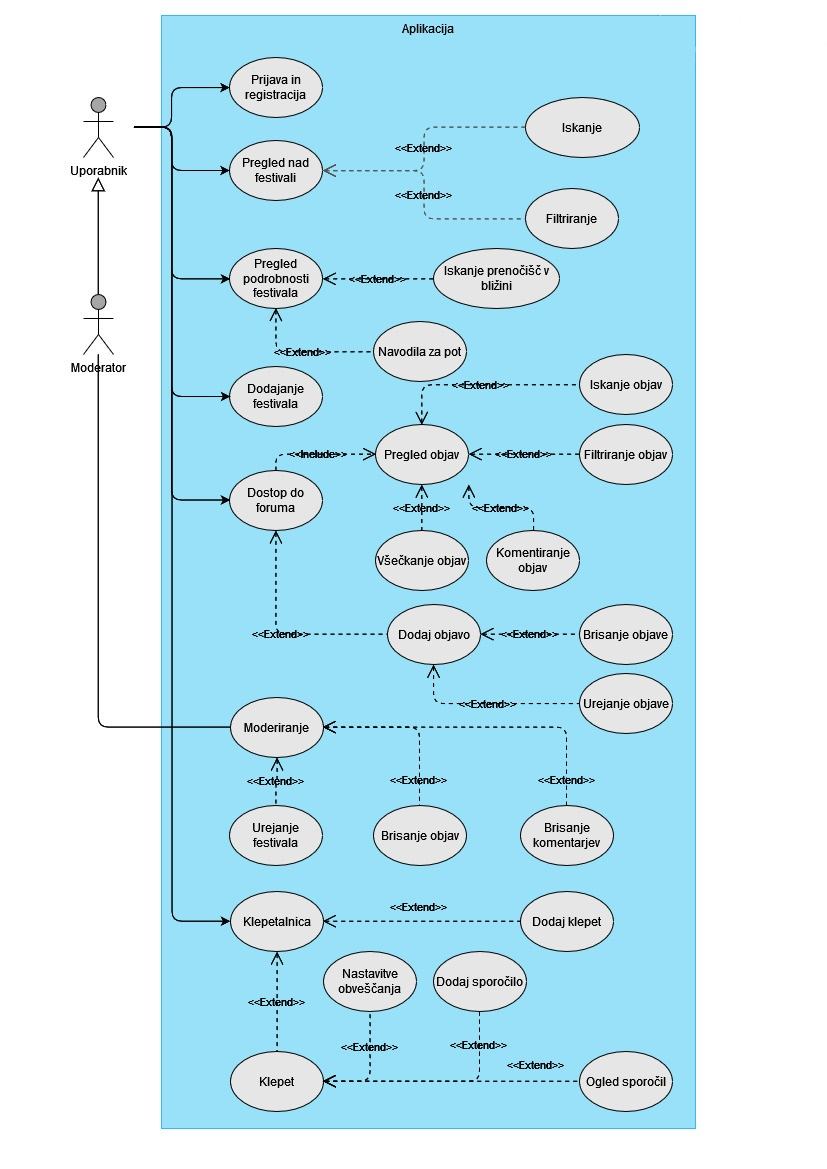
\includegraphics[width=0.99\textwidth]{img/UseCase}
\end{center}
\caption{Diagram primerov uporabe.}
\label{usecase}
\end{figure}

% NOVO POGLAVJE
\chapter{Uporabljene tehnologije in orodja}
Odločili smo se za uporabo modernih, dobro poznanih in pogosto uporabljenih tehnologij in orodij. Za čelni del smo uporabili
Nuxt \cite{nuxtintro}, ki temelji na ogrodju Vue.js \cite{vuejs}. Za zaledni del smo izbrali Django \cite{django} s knjižnico Django REST Framework \cite{drf}, 
ki močno olajša razvoj API vmesnikov in upravljanje s podatkovno bazo. Za podatkovno bazo smo uporabili PostgreSQL \cite{postgre}.
Realnočasovno komunikacijo smo omogočili s pomočjo Pusher Channels \cite{pusher}. Zemljevidi 
in navodila za pot so osnovani na platformi Mapbox \cite{mapbox}. Podatkovno bazo ter Django strežnik smo poganjali v Dockerju \cite{docker}.
Vse te tehnologije in orodja ter njihov namen in uporabo v naši rešitvi smo podrobneje predstavili v naslednjem poglavju.

Poleg omenjenih glavnih tehnologij smo sicer uporabili še Vuetify.js za oblikovanje spletne strani \cite{vuetify},
ter Git \cite{git} in GitHub \cite{github} za nadzor različic, za shranjevanje slik smo se odločili za Firebase Storage \cite{firebase}, za urejanje kode pa 
smo uporabljali Visual Studio Code \cite{vscode}. Poleg tega smo uporabili nekaj Python knjižnic, med njimi BeautifulSoup4 \cite{bs4} za strganje podatkov iz bookinga,
ter Djoser \cite{djoser}, ki ponuja vnaprej definirane končne točke za registracijo, prijavo, odjavo in aktivacijo uporabniškega računa. 

\section{Nuxt.js}
Nuxt.js (na kratko Nuxt) je brezplačno odprtokodno orodje za razvoj čelnega dela spletnih aplikacij z Vue.js. V naši aplikaciji smo ga uporabili zato, ker 
omogoča hiter, enostaven, predvsem pa učinkovit razvoj aplikacij. 

Poleg tega Nuxt nudi tudi SSR (Server-Side Rendering), ki omogoča hitrejše čase nalaganja strani in SEO (Search Engine Optimization). Pri tem strežnik po začetni zahtevi odjemalca 
pošlje v celoti renderirano stran nazaj odjemalcu. JavaScript na strani odjemalca nato omogoči, da statična stran postane interaktivna Vue.js aplikacija (hidracija) \cite{hydration}.

Ena večjih prednosti je tudi enostavna konfiguracija poti na spletni strani, saj Nuxt samodejno razbere strukturo glede na vsebino mape pages/. 
V Vue.js npr. je za vsako novo dodano stran to potrebno storiti ročno.

\section{Django in DRF}
Django je Python ogrodje za razvoj spletnih aplikacij, ustvarjeno z namenom da uporabniku omogoči hiter razvoj, s tem, da vsebuje širok nabor orodij,
ki poskrbijo za pogosto uporabljena opravila spletnega razvoja (avtentikacija, administracija, upravljanje z podatkovno bazo...).
Temelji na vzorcu Model-View-Template, ki je v osnovi zelo podoben bolj znanemu Model-View-Controller. Model skrbi za podatke in vzdržuje povezavo s podatkovno bazo.
View sprejema zahtevke in vrača odgovore, Template pa definira strukturo in postavitev strani, tipično z uporabo DTL (Django Template Language) \cite{mvt}.

Django REST Framework je razširitev za Django, posebej namenjena za gradnjo RESTful API-jev. V naši aplikaciji smo DRF v uporabili predvsem zaradi 
enostavnega dela s podatkovno bazo, enostavne serializacije podatkov (pretvorba kompleksnih podatkovnih tipov kot so Django modeli in poizvedbe v
format JSON ali XMl) in že vnaprej pripravljenih pogledov za nekatere osnovne CRUD operacije, 
ki jih z lahkoto lahko priredimo za naše namene. Poleg tega omogoča tudi enostavno pisanje pravic za dostop do API končnih točk.

\section{PostgreSQL}
Za podatkovno bazo smo uporabili PostgreSQL. PostgreSQL je zmogljiv odprtokoden objektno-relacijski DBMS (sistem za upravljanje s podatkovnimi bazami). Kljub temu, da je
odprtokoden se lahko kosa z ostalimi ponudniki, kot sta npr. Oracle in MySQL. Prav zaradi stroškov, se zelo pogosto uporablja v različnih startupih in za v 
raziskovalne namene \cite{juba2015learning}.

\section{Pusher Channels}
Realnočasovno komunikacijo v klepetih smo zagotovili s pomočjo storitve Pusher Channels. Pusher Channels deluje na tehnologiji WebSockets, ki omogoča vztrajne TCP povezave
med strežnikom in odjemalcem. S tem lahko strežnik in odjemalec dosežeta takojšnjo izmenjavo sporočil na zelo učinkovit način z majhno zakasnitvijo, brez da bi odjemalec
poslal zahtevo za prejem podatkov \cite{websockets}.

Pusher Channels delujejo na modelu objavi/naroči. Aplikacije se lahko naročajo na kanale v sistemu. Ko pride do sprememb, pa sistem objavi spremembo v ta isti kanal.
Vse aplikacije naročene na ta kanal, so potem obveščene \cite{pusher}.

\section{Mapbox}
Mapbox je spletna platforma, ki razvijalcem ponuja širok nabor orodij za delo z zemljevidi. Podatke črpa iz različnih virov, med drugim tudi iz MapStreetBoxa in NASE. 
V naši aplikaciji smo uporabili večino glavnih storitev, ki jih omogoča in sicer \cite{mapboxservices}:
\begin{itemize}
    \item \textbf{Mapbox Maps}, ki omogoča prikaz zemljevidov po meri z lokacijami. V naši aplikaciji prikazuje vse zemljevide.
    \item \textbf{Mapbox Directions API}, ki omogoča iskanje poti. V naši aplikaciji služi izrisovanju poti od vnešene lokacije do festivala.
    \item \textbf{Geocoding API}, ki spreminja koordinate v naslove in obratno. V naši aplikaciji je uporabljen, da koordinate pretvori v človeku prijazno predstavitev.
    \item \textbf{Mapbox Search Box}, ki omogoča iskanje lokacij. V naši aplikaciji je uporabljen za iskanje začetnih lokacij pri navigaciji in za interaktivno iskanje po zemljevidu.
\end{itemize}

\section{Docker}
Docker je platforma, ki omogoča ustvarjanje, izvajanje in nameščanje aplikacij v kontejnerjih/vsebnikih. Temu procesu pravimo kontejnerizacija.
Pri kontejnerizaciji zapakiramo programsko kodo s knjižnicami operacijskega sistema in odvisnostmi, ki so potrebne za izvajanje kode.
S tem ustvarimo lahko izvedljivo datoteko, ki se lahko enako izvaja na kateri koli infrastrukturi \cite{containerization}.
Prednosti uporabe Dockerja je veliko, v našem primeru pa smo ga uporabili predvsem zaradi izolacije okolja in lahke prenosljivosti.
V Dockerju smo poganjali Django aplikacijo ter podatkovno bazo.

% NOVO POGLAVJE
\chapter{Razvoj rešitve}
V tem poglavju bomo predstavili celoten proces razvoja naše rešitve, od začetnega načrtovanja arhitekture in podatkovne baze, do končne rešitve.
Pri tem se bomo posvetili predvsem na podatkovno bazo, implementacijo nekaterih glavnih funkcij aplikacije ter uporabniški vmesnik.

\section{Arhitektura aplikacije}

\begin{figure}[htb] % OPTIONS h-here, t-top, b-bottom, p-page
\begin{center}
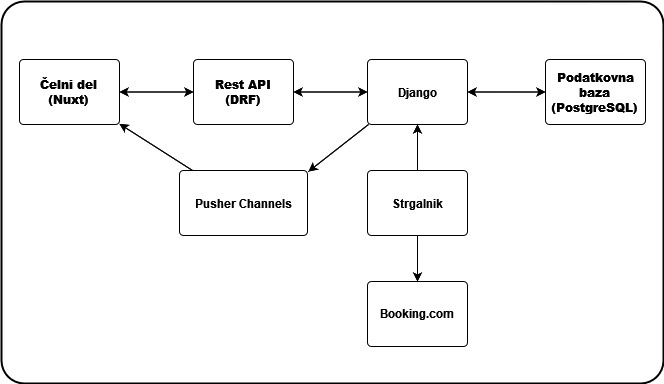
\includegraphics[width=\textwidth]{img/Architecture}
\end{center}
\caption{Arhitektura razvite rešitve.}
\label{architecture}
\end{figure}

Spletna aplikacija je sestavljena iz čelnega dela, kateri podatke pridobiva preko APIja implementiranega v Django Rest Frameworku.
V zalednem delu Django ORM skrbi za upravljanje s podatkovnimi modeli in poizvedbami.
Poleg tega skrbi za strganje podatkov o prenočiščih iz spletne strani Booking.com.
Prav tako pa Django ob vsakem dodanem sporočilu v klepetih pošlje obvestilo s pomočjo Pusher Channels na čelni del aplikacije, da se uporabniku na drugi strani le to takoj prikaže.

Na Sliki \ref{architecture} je prikazana arhitektura naše rešitve.

\section{Podatkovni model}
% - 1. kratek opis
% - 2. slika
% - 3. vsak model razloži

\section{Zaledni del}
% - 1. na kratko kaj mamo u Djangu (views, models) in kaj v drf(serializers) in zakaj smo uporabili, ku funkcionira ORM
Za implementacijo zalednega dela smo uporabili Django v kombinaciji z Django Rest Framework.

Django nam je omogočil poenostavljeno delo s podatkovno bazo, saj nam z vgrajenim ORM sistemom, ni potrebno pisati SQL stavkov, temveč lahko kodiramo v Pythonu.
To naredi vsako interakcijo s podatkovno bazo lažjo in bolj intuitivno, istočasno pa ne rabimo skrbeti glede SQL napadov, saj ORM vsako poizvedbo sestavi s poudarkom na varnosti. 

Knjižnica Django Rest Framework pa nam je z orodji za serializacijo, avtentikacijo in generičnimi pogledi, še dodatno olajšala implementacijo REST APIja.

% - 2. primer modela, viewa in serializera in url, avtentikacijska pravila
\subsection{Delo s podatkovno bazo}
Uporaba Django ORM nam je omogočila lahko povezavo z zalednim delom aplikacije.
V datoteki models.py smo definirali modele.
Modeli v Djangu predstavljajo strukturo in relacije v podatkovni bazi.
Vsak model predstavlja eno tabelo, vsak atribut pa eno polje v podatkovni bazi.
Django ORM potem samodejno poskrbi za kreacijo tabel glede na modele, vendar je potrebno najprej pognati ukaz \textit{python manage.py makemigrations}, da se ustvarijo migracije za vse spremembe.
Da se spremembe v datoteki z migracijami dejansko uporabijo in posodobijo podatkovno bazo, pa je potrebno pognati še ukaz \textit{python manage.py migrate}.

V spodnji Izvorni kodi~\ref{code1} je prikazano, kako smo definirali model za \textit{Festival}.
Z opcijo \textit{blank} definiramo, da v zahtevku s čelnega dela ni potrebno navesti določenega polja.
Z \textit{null} pa definiramo, da je lahko polje v podatkovni bazi NULL.
Polje \textit{genre} je povezava na tabelo Genre.
Z \textit{models.SET\_NULL} smo določili, da se ob primeru izbrisa instance žanra v festivalih povezanih s tem žanrom polje \textit{genre} postavi na NULL.
V razredu Meta pa smo določili, da so ob poizvedbah festivali po privzetem v vrstnem redu glede na polje \textit{name}.

\begin{lstlisting}[label=code1,caption=Primer kreiranja modela \textit{Festival} v Djangu.,frame=tb,captionpos=b]
class Festival(models.Model):
    name = models.CharField(max_length=50)
    info = models.TextField(
        blank=True, 
        default='No info provided'
    )
    website = models.URLField(
        blank=True,
        default='No website provided'
    )
    lat = models.FloatField(blank=True, null=True)
    lon = models.FloatField(blank=True, null=True)
    date_start = models.DateField(blank=True, null=True)
    date_end = models.DateField(blank=True, null=True)
    img = models.URLField(blank=True, null=True)

    genre = models.ForeignKey(
        Genre, 
        on_delete=models.SET_NULL, 
        null=True, 
        blank=True
    )

    class Meta:
        ordering = ['name']
\end{lstlisting}

\subsection{API}
Kot smo že omenili v uvodu v poglavje, smo za komunikacijo čelnega dela aplikacije z zalednim implementirali RESTful API s pomočjo Django Rest Frameworka.
Na zahteve odjemalca posluša na vratih 8000.

DRF močno pospeši izgradnjo APIjev, saj je za serializacijo podatkov potrebno le definirati razred za vsak model, ter našteti katera polja bomo serializirali.
S tem povemo, kako naj bodo polja modela predstavljena v obliki JSON, ki je standardni format za APIje.
Poleg osnovnih polj lahko serializiramo tudi izpeljana polja, ki niso neposredno na voljo v modelu.
To lahko naredimo tako, da definiramo metodo za izračun vrednosti.

V Izvorni kodi~\ref{code2} lahko vidimo primer serializacije podatkov za model \textit{Festival} s tremi dodatnimi izpeljanimi vrednostmi, ki jih izračunajo metode:
\begin{itemize}
    \item \textbf{is\_favourite} - Glede na uporabnika, ki zahteva podatke in izbrani festival, vrne vrednost True ali False glede na to ali ima uporabnik festival dodan med priljubljene.
    \item \textbf{get\_is\_mod} - Glede na uporabnika, ki zahteva podatke in izbrani festival, vrne vrednost True ali False glede na to ali je uporabnik moderator festivala.
    \item \textbf{get\_num\_favourites} - Glede na izbrani festival, vrne število vseh uporabnikov, ki imajo festival dodan med priljubljene.
\end{itemize}

\begin{lstlisting}[label=code2,caption=Primer serializacije podatkov za model \textit{Festival}.,frame=tb,captionpos=b]
class FestivalSerializer(serializers.ModelSerializer):
    is_favourite = serializers.SerializerMethodField()
    is_mod = serializers.SerializerMethodField()
    num_favourites = serializers.SerializerMethodField()

    class Meta:
        model = Festival
        fields = ['id', 
                    'name', 
                    'info', 
                    'website', 
                    'lat', 
                    'lon',
                    'date_start',
                    'date_end',
                    'img',
                    'genre',
                    
                    'is_mod',
                    'is_favourite',
                    'num_favourites']
        
        def get_is_favourite(self, obj):
            user = self.context['request'].user
            return user in obj.favourite_by.all()
        
        def get_is_mod(self, obj):
            user = self.context['request'].user
            return user in obj.mods.all()
        
        def get_num_favourites(self, obj):
            return len(obj.favourite_by.all())
\end{lstlisting}

Poleg serializacije podatkov, DRF omogoča tudi tako imenovane generične poglede (Generic Views).
Ti pogledi ponujajo pogosto uporabljene vzorce operacij CRUD na modelih in s tem poenostavijo proces grajenja APIja tako, da se zmanjšajo potrebo po pisanju ponavljajoče kode.
Prav tako omogočajo uporabo predefiniranih razredov s pravicami dostopa, iskanje po poljih modela ter paginacijo.
V Izvorni kodi~\ref{code3} lahko vidimo primer generičnega pogleda \textit{ListCreateAPIView}, ki ponuja končne točke za operacije GET in POST.
Preko te končne točke, lahko torej dostopamo do seznama vseh festivalov s filtri in opcijo iskanja ter določitve vrstnega reda rezultatov.
Lahko pa na tej točki tudi kreiramo nov festival.

\begin{lstlisting}[label=code3,caption=Primer pogleda za model \textit{Festival}\, ki omogoča kreiranje\, iskanje in vračanje festivalov urejenih po popularnosti in datumu.,frame=tb,captionpos=b]
class FestivalList(generics.ListCreateAPIView):
    permission_classes = (IsAuthenticated,)
    serializer_class = FestivalSerializer
    filter_backends = [SearchFilter]
    search_fields = ['name']

    def perform_create(self, serializer):
        festival = serializer.save()
        festival.mods.add(self.request.user)

    def get_queryset(self):
        order_by = self.request.query_params.get('order')

        queryset = Festival.objects.all()
        user = self.request.user
        if order_by == 'Popularity':
            queryset = queryset.annotate(
                most_popular=Count('favourite_by')
                )
                .all()
                .order_by('-most_popular')
        else:
            queryset = queryset.order_by(
                F('date_start').desc(nulls_last=True)
            )
    ...
\end{lstlisting}

Za delovanje APIja je potrebno poleg definicije modela, serializacije in pogleda za definirati še URL končne točke.
To lahko storimo v datoteki \textit{urls.py}, kjer definiramo URL naslov za vsako točko.
V naši aplikaciji smo poleg končnih točk za avtentikacijo implementirali 10 končnih točk in sicer:
\begin{itemize}
    \item \texttt{festivals/}
    \item \texttt{festivals/\{int:pk\}}
    \item \texttt{hotels/}
    \item \texttt{festivals/\{int:pk\}/chats/}
    \item \texttt{festivals/\{int:pk\}/chats/\{int:cpk\}}
    \item \texttt{notifications/}
    \item \texttt{posts/}
    \item \texttt{posts/\{int:pk\}}
    \item \texttt{posts/\{int:pk\}/comments}
    \item \texttt{comments/\{int:pk\}}
\end{itemize}

\subsection{Strgalnik}
Ena glavnih funkcij našega sistema je, da uporabniku omogoča prikaz preno\-čišč v bližini glasbenega festivala.
Za implementacijo je bilo potrebno najprej ugotoviti, s kje bo naša aplikacija črpala podatke.
Najlažje bi bilo, da bi obstajala storitev, ki bi ponujala brezplačen API, preko katerega bi lahko dostopali do podatkov, ki jih potrebujemo.
Izkazalo se je, da nobena izmed storitev, ki bi nam ustrezala, tega ne ponuja.
Za dostop do APIja spletnih strani Booking.com in Airbnb je tako potrebno čez dolgotrajen proces, po katerem šele lahko potem postanemo uradni partner.

Zaradi navedenega problema smo se odločili, da bomo podatke strgali iz spletne strani Booking.com.
Strganje podatkov smo izvedli s pomočjo Python knjižnice BeautifulSoup4.
Uporabnik na čelni strani pri izbranem festivalu vnese parametre za iskanje.
Na podlagi teh parametrov potem na zalednem delu skripta sestavi URL naslov, v taki obliki, kot če bi brskali po Bookingu, ter prebere vsebino strani in vrne rezultat v obliki JSON nazaj na čelni del.

\section{Implementacija Mapbox zemljevida}
Vsi zemljevidi so v celoti implementirani na čelnem delu aplikacije.
Preden lahko uporabljamo Mapbox je potrebno ustvariti uporabniški račun, da lahko pridobimo žeton za dostop.
Za osnoven zemljevid je potrebnih le nekaj vrstic kode, še pred tem pa je potrebno prenesti modul \textit{nuxt-mapbox}.
Nato ustvarimo novo instanco zemljevida, pri tem pa v osnovi dodamo naslednje vrednosti:
\begin{itemize}
    \item \textbf{container} - referenca na HTML element, ki bo vseboval zemljevid

    \item \textbf{style} - izbor izgleda zemljevida

    \item \textbf{center} - koordinate, ki bodo centrirane

    \item \textbf{zoom} - začetna povečava zemljevida

\end{itemize}

\begin{lstlisting}[label=code4,caption=Primer kode za prikaz lokacije na Mapbox zemljevidu.,frame=tb,captionpos=b]
new mapboxgl.Map({
    container: 'map',
    style: 'mapbox://styles/mapbox/outdoors-v12',
    center: [lon, lat],
    zoom: 16
})

let el = document.createElement('div')
el.className = 'marker img1'
const marker = new mapboxgl.Marker(el)
    .setLngLat([lon, lat])
    .addTo(map)
\end{lstlisting}

Bolj zanimiva pa je bila implementacija iskanja poti do festivala.
Za to smo uporabili Mapbox Directions API v kombinaciji z Mapbox Search Box vnosnim poljem.
Z uporabo Mapbox Directions API~\cite{mapboxdirections} smo lahko izračunali optimalne poti za vožnjo, ter prikazali navodila za pot do cilja.
Search Box pa omogoča, da uporabnik izbere izhodiščno lokacijo.

\subsection{Izbira izhodiščne lokacije}
Uporabnik lahko izhodiščno lokacijo izbere na 2 načina.
Pri prvem načinu uporabnik preko vnosnega polja Mapbox Search Box poišče lokacijo.
Ob izbiri, se sproži dogodek "retrieve", preko katerega lahko potem dostopamo do lokacije in izluščimo koordinate.

Druga opcija je, da uporabnik dovoli uporabo lokacije v aplikaciji.
Če to stori, lahko le s klikom na gumb pridobi pot od svoje trenutne lokacije do prizorišča.

Klic APIja izgleda tako:
\begin{lstlisting}[label=code5,caption=URL za klic Mapbox Directions APIja\, ki vrne navodila za pot v formatu GeoJSON.,frame=tb,captionpos=b]
const response = $fetch(
    `https://api.mapbox.com/directions/v5/mapbox/driving/
    ${startLocation.lon}%2C${startLocation.lat}%3B
    ${props.lon}%2C${props.lat}?
    alternatives=false
    &geometries=geojson
    &language=en
    &overview=simplified
    &steps=true
    &access_token=${runtimeConfig.public.mapboxToken}`
)
\end{lstlisting}

V odgovoru dobimo vsa navodila za vsak zavoj in vmesne točke, skupaj z pripadajočimi koordinatami.
Poleg tega dobimo tudi podatke o času trajanja vožnje v sekundah, ter dolžine poti v metrih.
Te podatke je potrebno nato še prikazati na zemljevidu.
To smo naredili z naslednjo kodo:
\begin{lstlisting}[label=code6,caption=Izvorna koda za prikaz poti na zemljevidu.,frame=tb,captionpos=b]
map.on('load', () => {
    map.addSource('route', {
        'type': 'geojson',
        'data': {
            'type': 'Feature',
            'properties': {},
            'geometry': {
                'type': 'LineString',
                'coordinates': props.directions.geoLines
            }
        }
    });
    map.addLayer({
        'id': 'route',
        'type': 'line',
        'source': 'route',
        'layout': {
            'line-join': 'round',
            'line-cap': 'round'
        },
        'paint': {
            'line-color': '#26A69A',
            'line-width': 5,
        }
    })
})
\end{lstlisting}

S tem smo dodali pot na zemljevid, vendar je bilo potrebno potem ponovno centrirati zemljevid tako, da je vidna celotna pot.
\begin{lstlisting}[label=code7,caption=Prilagoditev središča zemljevida in stopnje povečave\, da ustreza geografskemu območju poti.,frame=tb,captionpos=b]
const bounds = new mapboxgl.LngLatBounds()
props.directions.geoLines.forEach(([lon, lat]) => {
    bounds.extend([lon, lat])
})

const padding = { top: 50, bottom: 50, left: 50, right: 50 }
map.fitBounds(
    bounds,
    { padding }
)
\end{lstlisting}

\section{Realnočasovna komunikacija}
Pri implementaciji klepetov smo morali zagotoviti, da vsi uporabniki, ki so aktivni v določenem klepetu, prejmejo novo sporočilo takoj.
To smo dosegli z uporabo Pusher Channels, ki sloni na tehnologiji WebSockets.
Kako smo to vključili v naš sistem pa bomo opisali v naslednjem poglavju.

Za delovanje Pusher Channels smo najprej namestili knjižnici \textbf{pusher} na zalednem delu ter \textbf{pusher-js} na čelnem delu.
Potem smo ustvarili Pusher račun, da smo lahko pridobili pooblastila za uporabo Pusherja - \textit{app\_id, key in secret}.
Na zalednem delu smo potem ustvarili novo datoteko s kodo, ki inicializira novo instanco Pusherja.
Podobno smo storili tudi na čelnem delu, kjer pa je bilo potrebno kot parameter podati le \textit{key}.
\begin{lstlisting}[label=code8,caption=Izvorna koda\, ki kreira novo instanco Pusherja na zalednem delu.,frame=tb,captionpos=b]
import pusher, os

pusher = pusher.Pusher(
    app_id=os.environ.get('PUSHER_APP_ID'),
    key=os.environ.get('PUSHER_KEY'),
    secret=os.environ.get('PUSHER_SECRET'),
    cluster='eu',
    ssl=False
)    
\end{lstlisting}

\subsection{Sporočila}
Najprej smo implementirali realnočasovno sporočanje.
Za začetek smo metodo \textit{perform\_create} v pogledu MessageList prilagodili tako, da poleg kreiranja novega objekta in shrambe v podatkovno bazo, takoj odda sporočilo vsem prijavljenim v kanalu klepeta.
Potrebno je bilo podati ime kanala, ime dogodka (novo sporočilo), ter vsebino samega sporočila.
\begin{lstlisting}[label=code9,caption=Pošiljanje novega sporočila vsem odjemalcem naročenim na kanal chat-{message.chat.id} z uporabo storitve Pusher.,frame=tb,captionpos=b]
pusher.trigger(
    f'chat-{message.chat.id}',
    'new-message',
    data
)
\end{lstlisting}

S tem smo pokrili zaledni del, implementirati pa je bilo potrebno še prejemanje teh sporočil na čelnem delu.
To smo naredili tako, da smo najprej ustvarili Nuxt vtičnik z instanco Pusherja.
Do tega vtičnika smo potem lahko dostopali preko celotne aplikacije in preprečili možnost, da bi brez potrebe kreirali več instanc Pusherja, kot bi potrebovali.
To nam je tudi omogočilo, da smo z eno instanco Pusherja upravljali tako nova sporočila, kot obvestila.
\begin{lstlisting}[label=code10,caption=Nuxt vtičnik za novo instanco Pusherja.,frame=tb,captionpos=b]
import Pusher from 'pusher-js'

export default defineNuxtPlugin(nuxtApp => {
    const pusher = new Pusher(runtimeConfig.public.pusherKey, {
        cluster: 'eu'
    })

    nuxtApp.provide('pusher', pusher)
})
\end{lstlisting}
Vse kar je bilo potem še potrebno je bilo poslušati na nova sporočila.
Za to se je bilo potrebno naročiti na kanal za določen klepet, ter poslušati na dogodek 'new-message'.
\begin{lstlisting}[label=code11,caption=Poslušanje na nova sporočila na čelnem delu.,frame=tb,captionpos=b]
const channel = useNuxtApp().$pusher.subscribe(`chat-${chatId}`)       
channel.bind('new-message', (data) => {
    apiMessages.value.push(data)
})
\end{lstlisting}

\subsection{Notifikacije}
Podobno kot smo implementirali prejemanje sporočil v realnem času, smo implementirali tudi obvestila za prejeta sporočila.
Razlika je bila le ta, da smo najprej iterirali čez vse klepete (za katere ima uporabnik vklopljena obvestila) in se za vsakega posebej naročili na nov kanal.

\section{Večnivojski komentarji}
Implementacija foruma, je bila časovno najbolj potratna, zaradi velikega števila funkcionalnosti, ki jih podpira.
Za delovanje foruma smo v Djangu potrebovali modele CustomUser, Festival, Post in Comment, ter vse potrebne vmesne modele za všečkanje objav in komentarjev.

Problem, ki se je pojavil pri implementaciji foruma, je bil ta, kako omogočiti večnivojsko komentiranje.


\chapter{Uporabniški vmesnik}
\label{UI}

% - 3. nekaj skrinov slik uporabniškega vmesnika
%% -- pri vsakem potem npr. opises filtre, možnosti itd.

% TODO - neki od večnivojskih komentarju napisi

\chapter{Zaključek}

\section{Nadaljnji razvoj}
Zaradi kompleksnosti projekta, je možnosti za nadgradnje projekta veliko. 


%\cleardoublepage
%\addcontentsline{toc}{chapter}{Literatura}

% če imaš težave poravnati desni rob bibliografije, potem odkomentiraj spodnjo vrstico
\raggedright

\printbibliography[heading=bibintoc,type=article,title={Članki v revijah}]

\printbibliography[heading=bibintoc,type=inproceedings,title={Članki v zbornikih}]

\printbibliography[heading=bibintoc,type=incollection,title={Poglavja v knjigah}]

% v zadnji verziji diplomskega dela običajno združiš vse tri vrste referenc v en sam seznam in
% izpustiš delne sezname
\printbibliography[heading=bibintoc,title={Literatura}]

\end{document}

